
% Default to the notebook output style

    


% Inherit from the specified cell style.




    
\documentclass[11pt]{article}

    
    
    \usepackage[T1]{fontenc}
    % Nicer default font (+ math font) than Computer Modern for most use cases
    \usepackage{mathpazo}

    % Basic figure setup, for now with no caption control since it's done
    % automatically by Pandoc (which extracts ![](path) syntax from Markdown).
    \usepackage{graphicx}
    % We will generate all images so they have a width \maxwidth. This means
    % that they will get their normal width if they fit onto the page, but
    % are scaled down if they would overflow the margins.
    \makeatletter
    \def\maxwidth{\ifdim\Gin@nat@width>\linewidth\linewidth
    \else\Gin@nat@width\fi}
    \makeatother
    \let\Oldincludegraphics\includegraphics
    % Set max figure width to be 80% of text width, for now hardcoded.
    \renewcommand{\includegraphics}[1]{\Oldincludegraphics[width=.8\maxwidth]{#1}}
    % Ensure that by default, figures have no caption (until we provide a
    % proper Figure object with a Caption API and a way to capture that
    % in the conversion process - todo).
    \usepackage{caption}
    \DeclareCaptionLabelFormat{nolabel}{}
    \captionsetup{labelformat=nolabel}

    \usepackage{adjustbox} % Used to constrain images to a maximum size 
    \usepackage{xcolor} % Allow colors to be defined
    \usepackage{enumerate} % Needed for markdown enumerations to work
    \usepackage{geometry} % Used to adjust the document margins
    \usepackage{amsmath} % Equations
    \usepackage{amssymb} % Equations
    \usepackage{textcomp} % defines textquotesingle
    % Hack from http://tex.stackexchange.com/a/47451/13684:
    \AtBeginDocument{%
        \def\PYZsq{\textquotesingle}% Upright quotes in Pygmentized code
    }
    \usepackage{upquote} % Upright quotes for verbatim code
    \usepackage{eurosym} % defines \euro
    \usepackage[mathletters]{ucs} % Extended unicode (utf-8) support
    \usepackage[utf8x]{inputenc} % Allow utf-8 characters in the tex document
    \usepackage{fancyvrb} % verbatim replacement that allows latex
    \usepackage{grffile} % extends the file name processing of package graphics 
                         % to support a larger range 
    % The hyperref package gives us a pdf with properly built
    % internal navigation ('pdf bookmarks' for the table of contents,
    % internal cross-reference links, web links for URLs, etc.)
    \usepackage{hyperref}
    \usepackage{longtable} % longtable support required by pandoc >1.10
    \usepackage{booktabs}  % table support for pandoc > 1.12.2
    \usepackage[inline]{enumitem} % IRkernel/repr support (it uses the enumerate* environment)
    \usepackage[normalem]{ulem} % ulem is needed to support strikethroughs (\sout)
                                % normalem makes italics be italics, not underlines
    

    
    
    % Colors for the hyperref package
    \definecolor{urlcolor}{rgb}{0,.145,.698}
    \definecolor{linkcolor}{rgb}{.71,0.21,0.01}
    \definecolor{citecolor}{rgb}{.12,.54,.11}

    % ANSI colors
    \definecolor{ansi-black}{HTML}{3E424D}
    \definecolor{ansi-black-intense}{HTML}{282C36}
    \definecolor{ansi-red}{HTML}{E75C58}
    \definecolor{ansi-red-intense}{HTML}{B22B31}
    \definecolor{ansi-green}{HTML}{00A250}
    \definecolor{ansi-green-intense}{HTML}{007427}
    \definecolor{ansi-yellow}{HTML}{DDB62B}
    \definecolor{ansi-yellow-intense}{HTML}{B27D12}
    \definecolor{ansi-blue}{HTML}{208FFB}
    \definecolor{ansi-blue-intense}{HTML}{0065CA}
    \definecolor{ansi-magenta}{HTML}{D160C4}
    \definecolor{ansi-magenta-intense}{HTML}{A03196}
    \definecolor{ansi-cyan}{HTML}{60C6C8}
    \definecolor{ansi-cyan-intense}{HTML}{258F8F}
    \definecolor{ansi-white}{HTML}{C5C1B4}
    \definecolor{ansi-white-intense}{HTML}{A1A6B2}

    % commands and environments needed by pandoc snippets
    % extracted from the output of `pandoc -s`
    \providecommand{\tightlist}{%
      \setlength{\itemsep}{0pt}\setlength{\parskip}{0pt}}
    \DefineVerbatimEnvironment{Highlighting}{Verbatim}{commandchars=\\\{\}}
    % Add ',fontsize=\small' for more characters per line
    \newenvironment{Shaded}{}{}
    \newcommand{\KeywordTok}[1]{\textcolor[rgb]{0.00,0.44,0.13}{\textbf{{#1}}}}
    \newcommand{\DataTypeTok}[1]{\textcolor[rgb]{0.56,0.13,0.00}{{#1}}}
    \newcommand{\DecValTok}[1]{\textcolor[rgb]{0.25,0.63,0.44}{{#1}}}
    \newcommand{\BaseNTok}[1]{\textcolor[rgb]{0.25,0.63,0.44}{{#1}}}
    \newcommand{\FloatTok}[1]{\textcolor[rgb]{0.25,0.63,0.44}{{#1}}}
    \newcommand{\CharTok}[1]{\textcolor[rgb]{0.25,0.44,0.63}{{#1}}}
    \newcommand{\StringTok}[1]{\textcolor[rgb]{0.25,0.44,0.63}{{#1}}}
    \newcommand{\CommentTok}[1]{\textcolor[rgb]{0.38,0.63,0.69}{\textit{{#1}}}}
    \newcommand{\OtherTok}[1]{\textcolor[rgb]{0.00,0.44,0.13}{{#1}}}
    \newcommand{\AlertTok}[1]{\textcolor[rgb]{1.00,0.00,0.00}{\textbf{{#1}}}}
    \newcommand{\FunctionTok}[1]{\textcolor[rgb]{0.02,0.16,0.49}{{#1}}}
    \newcommand{\RegionMarkerTok}[1]{{#1}}
    \newcommand{\ErrorTok}[1]{\textcolor[rgb]{1.00,0.00,0.00}{\textbf{{#1}}}}
    \newcommand{\NormalTok}[1]{{#1}}
    
    % Additional commands for more recent versions of Pandoc
    \newcommand{\ConstantTok}[1]{\textcolor[rgb]{0.53,0.00,0.00}{{#1}}}
    \newcommand{\SpecialCharTok}[1]{\textcolor[rgb]{0.25,0.44,0.63}{{#1}}}
    \newcommand{\VerbatimStringTok}[1]{\textcolor[rgb]{0.25,0.44,0.63}{{#1}}}
    \newcommand{\SpecialStringTok}[1]{\textcolor[rgb]{0.73,0.40,0.53}{{#1}}}
    \newcommand{\ImportTok}[1]{{#1}}
    \newcommand{\DocumentationTok}[1]{\textcolor[rgb]{0.73,0.13,0.13}{\textit{{#1}}}}
    \newcommand{\AnnotationTok}[1]{\textcolor[rgb]{0.38,0.63,0.69}{\textbf{\textit{{#1}}}}}
    \newcommand{\CommentVarTok}[1]{\textcolor[rgb]{0.38,0.63,0.69}{\textbf{\textit{{#1}}}}}
    \newcommand{\VariableTok}[1]{\textcolor[rgb]{0.10,0.09,0.49}{{#1}}}
    \newcommand{\ControlFlowTok}[1]{\textcolor[rgb]{0.00,0.44,0.13}{\textbf{{#1}}}}
    \newcommand{\OperatorTok}[1]{\textcolor[rgb]{0.40,0.40,0.40}{{#1}}}
    \newcommand{\BuiltInTok}[1]{{#1}}
    \newcommand{\ExtensionTok}[1]{{#1}}
    \newcommand{\PreprocessorTok}[1]{\textcolor[rgb]{0.74,0.48,0.00}{{#1}}}
    \newcommand{\AttributeTok}[1]{\textcolor[rgb]{0.49,0.56,0.16}{{#1}}}
    \newcommand{\InformationTok}[1]{\textcolor[rgb]{0.38,0.63,0.69}{\textbf{\textit{{#1}}}}}
    \newcommand{\WarningTok}[1]{\textcolor[rgb]{0.38,0.63,0.69}{\textbf{\textit{{#1}}}}}
    
    
    % Define a nice break command that doesn't care if a line doesn't already
    % exist.
    \def\br{\hspace*{\fill} \\* }
    % Math Jax compatability definitions
    \def\gt{>}
    \def\lt{<}
    % Document parameters
    \title{Tutorial\_Session1}
    
    
    

    % Pygments definitions
    
\makeatletter
\def\PY@reset{\let\PY@it=\relax \let\PY@bf=\relax%
    \let\PY@ul=\relax \let\PY@tc=\relax%
    \let\PY@bc=\relax \let\PY@ff=\relax}
\def\PY@tok#1{\csname PY@tok@#1\endcsname}
\def\PY@toks#1+{\ifx\relax#1\empty\else%
    \PY@tok{#1}\expandafter\PY@toks\fi}
\def\PY@do#1{\PY@bc{\PY@tc{\PY@ul{%
    \PY@it{\PY@bf{\PY@ff{#1}}}}}}}
\def\PY#1#2{\PY@reset\PY@toks#1+\relax+\PY@do{#2}}

\expandafter\def\csname PY@tok@w\endcsname{\def\PY@tc##1{\textcolor[rgb]{0.73,0.73,0.73}{##1}}}
\expandafter\def\csname PY@tok@c\endcsname{\let\PY@it=\textit\def\PY@tc##1{\textcolor[rgb]{0.25,0.50,0.50}{##1}}}
\expandafter\def\csname PY@tok@cp\endcsname{\def\PY@tc##1{\textcolor[rgb]{0.74,0.48,0.00}{##1}}}
\expandafter\def\csname PY@tok@k\endcsname{\let\PY@bf=\textbf\def\PY@tc##1{\textcolor[rgb]{0.00,0.50,0.00}{##1}}}
\expandafter\def\csname PY@tok@kp\endcsname{\def\PY@tc##1{\textcolor[rgb]{0.00,0.50,0.00}{##1}}}
\expandafter\def\csname PY@tok@kt\endcsname{\def\PY@tc##1{\textcolor[rgb]{0.69,0.00,0.25}{##1}}}
\expandafter\def\csname PY@tok@o\endcsname{\def\PY@tc##1{\textcolor[rgb]{0.40,0.40,0.40}{##1}}}
\expandafter\def\csname PY@tok@ow\endcsname{\let\PY@bf=\textbf\def\PY@tc##1{\textcolor[rgb]{0.67,0.13,1.00}{##1}}}
\expandafter\def\csname PY@tok@nb\endcsname{\def\PY@tc##1{\textcolor[rgb]{0.00,0.50,0.00}{##1}}}
\expandafter\def\csname PY@tok@nf\endcsname{\def\PY@tc##1{\textcolor[rgb]{0.00,0.00,1.00}{##1}}}
\expandafter\def\csname PY@tok@nc\endcsname{\let\PY@bf=\textbf\def\PY@tc##1{\textcolor[rgb]{0.00,0.00,1.00}{##1}}}
\expandafter\def\csname PY@tok@nn\endcsname{\let\PY@bf=\textbf\def\PY@tc##1{\textcolor[rgb]{0.00,0.00,1.00}{##1}}}
\expandafter\def\csname PY@tok@ne\endcsname{\let\PY@bf=\textbf\def\PY@tc##1{\textcolor[rgb]{0.82,0.25,0.23}{##1}}}
\expandafter\def\csname PY@tok@nv\endcsname{\def\PY@tc##1{\textcolor[rgb]{0.10,0.09,0.49}{##1}}}
\expandafter\def\csname PY@tok@no\endcsname{\def\PY@tc##1{\textcolor[rgb]{0.53,0.00,0.00}{##1}}}
\expandafter\def\csname PY@tok@nl\endcsname{\def\PY@tc##1{\textcolor[rgb]{0.63,0.63,0.00}{##1}}}
\expandafter\def\csname PY@tok@ni\endcsname{\let\PY@bf=\textbf\def\PY@tc##1{\textcolor[rgb]{0.60,0.60,0.60}{##1}}}
\expandafter\def\csname PY@tok@na\endcsname{\def\PY@tc##1{\textcolor[rgb]{0.49,0.56,0.16}{##1}}}
\expandafter\def\csname PY@tok@nt\endcsname{\let\PY@bf=\textbf\def\PY@tc##1{\textcolor[rgb]{0.00,0.50,0.00}{##1}}}
\expandafter\def\csname PY@tok@nd\endcsname{\def\PY@tc##1{\textcolor[rgb]{0.67,0.13,1.00}{##1}}}
\expandafter\def\csname PY@tok@s\endcsname{\def\PY@tc##1{\textcolor[rgb]{0.73,0.13,0.13}{##1}}}
\expandafter\def\csname PY@tok@sd\endcsname{\let\PY@it=\textit\def\PY@tc##1{\textcolor[rgb]{0.73,0.13,0.13}{##1}}}
\expandafter\def\csname PY@tok@si\endcsname{\let\PY@bf=\textbf\def\PY@tc##1{\textcolor[rgb]{0.73,0.40,0.53}{##1}}}
\expandafter\def\csname PY@tok@se\endcsname{\let\PY@bf=\textbf\def\PY@tc##1{\textcolor[rgb]{0.73,0.40,0.13}{##1}}}
\expandafter\def\csname PY@tok@sr\endcsname{\def\PY@tc##1{\textcolor[rgb]{0.73,0.40,0.53}{##1}}}
\expandafter\def\csname PY@tok@ss\endcsname{\def\PY@tc##1{\textcolor[rgb]{0.10,0.09,0.49}{##1}}}
\expandafter\def\csname PY@tok@sx\endcsname{\def\PY@tc##1{\textcolor[rgb]{0.00,0.50,0.00}{##1}}}
\expandafter\def\csname PY@tok@m\endcsname{\def\PY@tc##1{\textcolor[rgb]{0.40,0.40,0.40}{##1}}}
\expandafter\def\csname PY@tok@gh\endcsname{\let\PY@bf=\textbf\def\PY@tc##1{\textcolor[rgb]{0.00,0.00,0.50}{##1}}}
\expandafter\def\csname PY@tok@gu\endcsname{\let\PY@bf=\textbf\def\PY@tc##1{\textcolor[rgb]{0.50,0.00,0.50}{##1}}}
\expandafter\def\csname PY@tok@gd\endcsname{\def\PY@tc##1{\textcolor[rgb]{0.63,0.00,0.00}{##1}}}
\expandafter\def\csname PY@tok@gi\endcsname{\def\PY@tc##1{\textcolor[rgb]{0.00,0.63,0.00}{##1}}}
\expandafter\def\csname PY@tok@gr\endcsname{\def\PY@tc##1{\textcolor[rgb]{1.00,0.00,0.00}{##1}}}
\expandafter\def\csname PY@tok@ge\endcsname{\let\PY@it=\textit}
\expandafter\def\csname PY@tok@gs\endcsname{\let\PY@bf=\textbf}
\expandafter\def\csname PY@tok@gp\endcsname{\let\PY@bf=\textbf\def\PY@tc##1{\textcolor[rgb]{0.00,0.00,0.50}{##1}}}
\expandafter\def\csname PY@tok@go\endcsname{\def\PY@tc##1{\textcolor[rgb]{0.53,0.53,0.53}{##1}}}
\expandafter\def\csname PY@tok@gt\endcsname{\def\PY@tc##1{\textcolor[rgb]{0.00,0.27,0.87}{##1}}}
\expandafter\def\csname PY@tok@err\endcsname{\def\PY@bc##1{\setlength{\fboxsep}{0pt}\fcolorbox[rgb]{1.00,0.00,0.00}{1,1,1}{\strut ##1}}}
\expandafter\def\csname PY@tok@kc\endcsname{\let\PY@bf=\textbf\def\PY@tc##1{\textcolor[rgb]{0.00,0.50,0.00}{##1}}}
\expandafter\def\csname PY@tok@kd\endcsname{\let\PY@bf=\textbf\def\PY@tc##1{\textcolor[rgb]{0.00,0.50,0.00}{##1}}}
\expandafter\def\csname PY@tok@kn\endcsname{\let\PY@bf=\textbf\def\PY@tc##1{\textcolor[rgb]{0.00,0.50,0.00}{##1}}}
\expandafter\def\csname PY@tok@kr\endcsname{\let\PY@bf=\textbf\def\PY@tc##1{\textcolor[rgb]{0.00,0.50,0.00}{##1}}}
\expandafter\def\csname PY@tok@bp\endcsname{\def\PY@tc##1{\textcolor[rgb]{0.00,0.50,0.00}{##1}}}
\expandafter\def\csname PY@tok@fm\endcsname{\def\PY@tc##1{\textcolor[rgb]{0.00,0.00,1.00}{##1}}}
\expandafter\def\csname PY@tok@vc\endcsname{\def\PY@tc##1{\textcolor[rgb]{0.10,0.09,0.49}{##1}}}
\expandafter\def\csname PY@tok@vg\endcsname{\def\PY@tc##1{\textcolor[rgb]{0.10,0.09,0.49}{##1}}}
\expandafter\def\csname PY@tok@vi\endcsname{\def\PY@tc##1{\textcolor[rgb]{0.10,0.09,0.49}{##1}}}
\expandafter\def\csname PY@tok@vm\endcsname{\def\PY@tc##1{\textcolor[rgb]{0.10,0.09,0.49}{##1}}}
\expandafter\def\csname PY@tok@sa\endcsname{\def\PY@tc##1{\textcolor[rgb]{0.73,0.13,0.13}{##1}}}
\expandafter\def\csname PY@tok@sb\endcsname{\def\PY@tc##1{\textcolor[rgb]{0.73,0.13,0.13}{##1}}}
\expandafter\def\csname PY@tok@sc\endcsname{\def\PY@tc##1{\textcolor[rgb]{0.73,0.13,0.13}{##1}}}
\expandafter\def\csname PY@tok@dl\endcsname{\def\PY@tc##1{\textcolor[rgb]{0.73,0.13,0.13}{##1}}}
\expandafter\def\csname PY@tok@s2\endcsname{\def\PY@tc##1{\textcolor[rgb]{0.73,0.13,0.13}{##1}}}
\expandafter\def\csname PY@tok@sh\endcsname{\def\PY@tc##1{\textcolor[rgb]{0.73,0.13,0.13}{##1}}}
\expandafter\def\csname PY@tok@s1\endcsname{\def\PY@tc##1{\textcolor[rgb]{0.73,0.13,0.13}{##1}}}
\expandafter\def\csname PY@tok@mb\endcsname{\def\PY@tc##1{\textcolor[rgb]{0.40,0.40,0.40}{##1}}}
\expandafter\def\csname PY@tok@mf\endcsname{\def\PY@tc##1{\textcolor[rgb]{0.40,0.40,0.40}{##1}}}
\expandafter\def\csname PY@tok@mh\endcsname{\def\PY@tc##1{\textcolor[rgb]{0.40,0.40,0.40}{##1}}}
\expandafter\def\csname PY@tok@mi\endcsname{\def\PY@tc##1{\textcolor[rgb]{0.40,0.40,0.40}{##1}}}
\expandafter\def\csname PY@tok@il\endcsname{\def\PY@tc##1{\textcolor[rgb]{0.40,0.40,0.40}{##1}}}
\expandafter\def\csname PY@tok@mo\endcsname{\def\PY@tc##1{\textcolor[rgb]{0.40,0.40,0.40}{##1}}}
\expandafter\def\csname PY@tok@ch\endcsname{\let\PY@it=\textit\def\PY@tc##1{\textcolor[rgb]{0.25,0.50,0.50}{##1}}}
\expandafter\def\csname PY@tok@cm\endcsname{\let\PY@it=\textit\def\PY@tc##1{\textcolor[rgb]{0.25,0.50,0.50}{##1}}}
\expandafter\def\csname PY@tok@cpf\endcsname{\let\PY@it=\textit\def\PY@tc##1{\textcolor[rgb]{0.25,0.50,0.50}{##1}}}
\expandafter\def\csname PY@tok@c1\endcsname{\let\PY@it=\textit\def\PY@tc##1{\textcolor[rgb]{0.25,0.50,0.50}{##1}}}
\expandafter\def\csname PY@tok@cs\endcsname{\let\PY@it=\textit\def\PY@tc##1{\textcolor[rgb]{0.25,0.50,0.50}{##1}}}

\def\PYZbs{\char`\\}
\def\PYZus{\char`\_}
\def\PYZob{\char`\{}
\def\PYZcb{\char`\}}
\def\PYZca{\char`\^}
\def\PYZam{\char`\&}
\def\PYZlt{\char`\<}
\def\PYZgt{\char`\>}
\def\PYZsh{\char`\#}
\def\PYZpc{\char`\%}
\def\PYZdl{\char`\$}
\def\PYZhy{\char`\-}
\def\PYZsq{\char`\'}
\def\PYZdq{\char`\"}
\def\PYZti{\char`\~}
% for compatibility with earlier versions
\def\PYZat{@}
\def\PYZlb{[}
\def\PYZrb{]}
\makeatother


    % Exact colors from NB
    \definecolor{incolor}{rgb}{0.0, 0.0, 0.5}
    \definecolor{outcolor}{rgb}{0.545, 0.0, 0.0}



    
    % Prevent overflowing lines due to hard-to-break entities
    \sloppy 
    % Setup hyperref package
    \hypersetup{
      breaklinks=true,  % so long urls are correctly broken across lines
      colorlinks=true,
      urlcolor=urlcolor,
      linkcolor=linkcolor,
      citecolor=citecolor,
      }
    % Slightly bigger margins than the latex defaults
    
    \geometry{verbose,tmargin=1in,bmargin=1in,lmargin=1in,rmargin=1in}
    
    

    \begin{document}
    
    
    \maketitle
    
    

    
    \begin{center}\rule{0.5\linewidth}{\linethickness}\end{center}

\section{\texorpdfstring{ \textbf{PYTHON} }{ PYTHON }}\label{python}

\begin{itemize}
\tightlist
\item
  Interactive, interpreted, and object-oriented programming language.
\item
  Simple syntax
\item
  Developed by Guido Van Rossum in 1991 at the National Research
  Institute for Mathematics and Computer Science in the Netherlands.
\item
  Name was inspired by: Monty Python's Flying Circus
\end{itemize}

    \subsection{ PYTHON PROGRAMMING ENVIRONMENT
}\label{python-programming-environment}

\begin{itemize}
\tightlist
\item
  Available on a wide variety of platforms including Windows, Linux and
  Mac OS X.
\item
  Official Website: \textbf{\href{https://python.org}{python.org}}
\item
  IDLE stands for Integrated Development and Learning Environment.
  Python IDLE comprises Python Shell and Python Editor. Python Shell
  Python Editor\\
  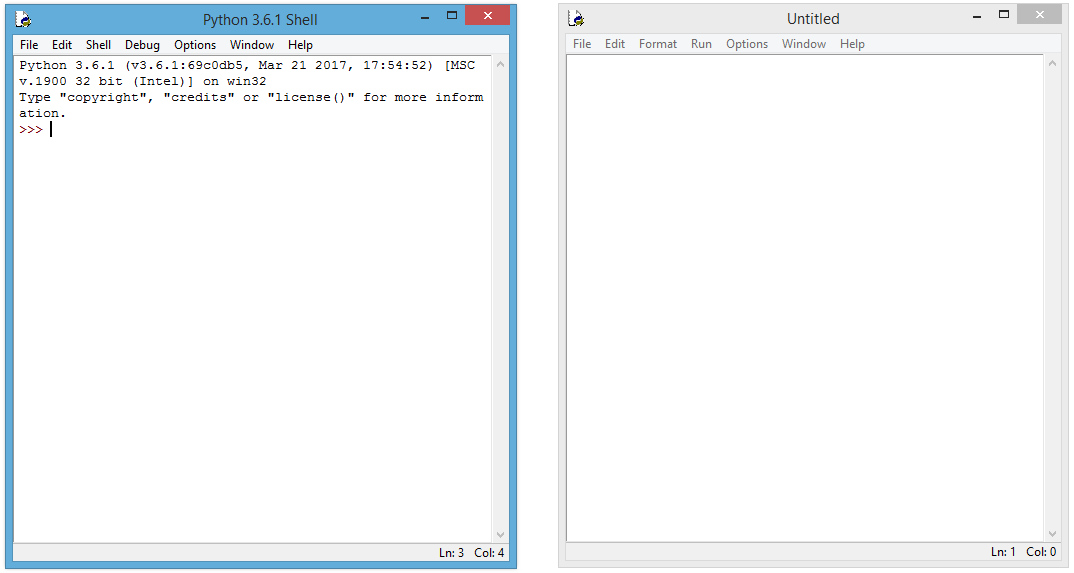
\includegraphics{1.png}
\end{itemize}

\begin{center}\rule{0.5\linewidth}{\linethickness}\end{center}

    \subsection{ Display on screen }\label{display-on-screen}

    \begin{Verbatim}[commandchars=\\\{\}]
{\color{incolor}In [{\color{incolor}2}]:} \PY{n+nb}{print}\PY{p}{(}\PY{l+s+s1}{\PYZsq{}}\PY{l+s+s1}{hello world}\PY{l+s+s1}{\PYZsq{}}\PY{p}{)}
\end{Verbatim}


    \begin{Verbatim}[commandchars=\\\{\}]
hello world

    \end{Verbatim}

    \begin{center}\rule{0.5\linewidth}{\linethickness}\end{center}

\subsection{ Names (Variables) and Assignment Statements
}\label{names-variables-and-assignment-statements}

\begin{itemize}
\tightlist
\item
  Variables provide a means to name values so that they can be used and
  manipulated later.
\item
  Assignment Statement: Statement that assigns value to a variable.
\end{itemize}

    \begin{Verbatim}[commandchars=\\\{\}]
{\color{incolor}In [{\color{incolor} }]:} \PY{n}{english} \PY{o}{=} \PY{l+m+mi}{57}
        \PY{n+nb}{print}\PY{p}{(}\PY{n}{english}\PY{p}{)}
\end{Verbatim}


    Python associates the \textbf{name} (variable) \textbf{english} with
value \textbf{57} i.e. the name (variable) \textbf{english} is assigned
the value \textbf{57}, or that the name (variable) \textbf{english}
refers to value \textbf{57}. Values are also called \textbf{objects}.


\includegraphics{2.png}

    \subsubsection{ Rules for creating a name (variable)
}\label{rules-for-creating-a-name-variable}

\begin{itemize}
\tightlist
\item
  Must begin with a letter or \_ (underscore character)
\item
  May contain any number of letters, digits, or underscore characters.
  No other character apart from these is allowed.
\end{itemize}

    \subsubsection{ Shorthand Notation }\label{shorthand-notation}

\begin{verbatim}
        a = a <operator> b            is equivalent to
        a <operator>= b
\end{verbatim}

    \begin{Verbatim}[commandchars=\\\{\}]
{\color{incolor}In [{\color{incolor}3}]:} \PY{n}{a} \PY{o}{=} \PY{l+m+mi}{6}
        \PY{n}{a} \PY{o}{=} \PY{n}{a} \PY{o}{+} \PY{l+m+mi}{5}
        \PY{n+nb}{print}\PY{p}{(}\PY{n}{a}\PY{p}{)}
        \PY{n}{a} \PY{o}{=} \PY{l+m+mi}{6}
        \PY{n}{a} \PY{o}{+}\PY{o}{=} \PY{l+m+mi}{5}
        \PY{n+nb}{print}\PY{p}{(}\PY{n}{a}\PY{p}{)}
\end{Verbatim}


    \begin{Verbatim}[commandchars=\\\{\}]
11
11

    \end{Verbatim}

    \subsubsection{ Multiple Assignments }\label{multiple-assignments}

\begin{itemize}
\tightlist
\item
  Used to enhance the readability of the program.
\end{itemize}

    \begin{Verbatim}[commandchars=\\\{\}]
{\color{incolor}In [{\color{incolor}7}]:} \PY{n}{msg}\PY{p}{,} \PY{n}{day}\PY{p}{,} \PY{n}{time} \PY{o}{=} \PY{l+s+s1}{\PYZsq{}}\PY{l+s+s1}{Meeting}\PY{l+s+s1}{\PYZsq{}}\PY{p}{,} \PY{l+s+s1}{\PYZsq{}}\PY{l+s+s1}{Mon}\PY{l+s+s1}{\PYZsq{}}\PY{p}{,} \PY{l+s+s1}{\PYZsq{}}\PY{l+s+s1}{9}\PY{l+s+s1}{\PYZsq{}}
        \PY{n}{totalMarks} \PY{o}{=} \PY{n}{count} \PY{o}{=} \PY{l+m+mi}{0}
\end{Verbatim}


    \begin{center}\rule{0.5\linewidth}{\linethickness}\end{center}

\subsection{ Arithmetic Operators }\label{arithmetic-operators}

    \begin{Verbatim}[commandchars=\\\{\}]
{\color{incolor}In [{\color{incolor}11}]:} \PY{n+nb}{print}\PY{p}{(}\PY{l+s+s2}{\PYZdq{}}\PY{l+s+s2}{18 + 5 =}\PY{l+s+s2}{\PYZdq{}}\PY{p}{,} \PY{l+m+mi}{18} \PY{o}{+} \PY{l+m+mi}{5}\PY{p}{)}    \PY{c+c1}{\PYZsh{}Addition}
         \PY{n+nb}{print}\PY{p}{(}\PY{l+s+s2}{\PYZdq{}}\PY{l+s+s2}{18 \PYZhy{} 5 =}\PY{l+s+s2}{\PYZdq{}}\PY{p}{,} \PY{l+m+mi}{18} \PY{o}{\PYZhy{}} \PY{l+m+mi}{5}\PY{p}{)}    \PY{c+c1}{\PYZsh{}Subtraction}
         \PY{n+nb}{print}\PY{p}{(}\PY{l+s+s2}{\PYZdq{}}\PY{l+s+s2}{18 * 5 =}\PY{l+s+s2}{\PYZdq{}}\PY{p}{,} \PY{l+m+mi}{18} \PY{o}{*} \PY{l+m+mi}{5}\PY{p}{)}    \PY{c+c1}{\PYZsh{}Multiplication}
         \PY{n+nb}{print}\PY{p}{(}\PY{l+s+s2}{\PYZdq{}}\PY{l+s+s2}{27 / 5 =}\PY{l+s+s2}{\PYZdq{}}\PY{p}{,} \PY{l+m+mi}{27} \PY{o}{/} \PY{l+m+mi}{5}\PY{p}{)}    \PY{c+c1}{\PYZsh{}Division}
         \PY{n+nb}{print}\PY{p}{(}\PY{l+s+s2}{\PYZdq{}}\PY{l+s+s2}{27 // 5 =}\PY{l+s+s2}{\PYZdq{}}\PY{p}{,} \PY{l+m+mi}{27} \PY{o}{/}\PY{o}{/} \PY{l+m+mi}{5}\PY{p}{)}  \PY{c+c1}{\PYZsh{}Integer Division}
         \PY{n+nb}{print}\PY{p}{(}\PY{l+s+s2}{\PYZdq{}}\PY{l+s+s2}{27 }\PY{l+s+s2}{\PYZpc{}}\PY{l+s+s2}{ 5 =}\PY{l+s+s2}{\PYZdq{}}\PY{p}{,} \PY{l+m+mi}{27} \PY{o}{\PYZpc{}} \PY{l+m+mi}{5}\PY{p}{)}    \PY{c+c1}{\PYZsh{}Modulus}
         \PY{n+nb}{print}\PY{p}{(}\PY{l+s+s2}{\PYZdq{}}\PY{l+s+s2}{2 ** 3 =}\PY{l+s+s2}{\PYZdq{}}\PY{p}{,} \PY{l+m+mi}{2} \PY{o}{*}\PY{o}{*} \PY{l+m+mi}{3}\PY{p}{)}    \PY{c+c1}{\PYZsh{}Exponentiation}
         \PY{n+nb}{print}\PY{p}{(}\PY{l+s+s2}{\PYZdq{}}\PY{l+s+s2}{\PYZhy{}2 ** 3 =}\PY{l+s+s2}{\PYZdq{}}\PY{p}{,} \PY{o}{\PYZhy{}}\PY{l+m+mi}{2} \PY{o}{*}\PY{o}{*} \PY{l+m+mi}{3}\PY{p}{)}  \PY{c+c1}{\PYZsh{}Exponentiation}
\end{Verbatim}


    \begin{Verbatim}[commandchars=\\\{\}]
18 + 5 = 23
18 - 5 = 13
18 * 5 = 90
27 / 5 = 5.4
27 // 5 = 5
27 \% 5 = 2
2 ** 3 = 8
-2 ** 3 = -8

    \end{Verbatim}

    \begin{Verbatim}[commandchars=\\\{\}]
{\color{incolor}In [{\color{incolor}9}]:} \PY{n+nb}{print}\PY{p}{(}\PY{l+s+s2}{\PYZdq{}}\PY{l+s+s2}{\PYZsq{}}\PY{l+s+s2}{how}\PY{l+s+s2}{\PYZsq{}}\PY{l+s+s2}{ + }\PY{l+s+s2}{\PYZsq{}}\PY{l+s+s2}{ are}\PY{l+s+s2}{\PYZsq{}}\PY{l+s+s2}{ + }\PY{l+s+s2}{\PYZsq{}}\PY{l+s+s2}{ you?}\PY{l+s+s2}{\PYZsq{}}\PY{l+s+s2}{:}\PY{l+s+s2}{\PYZdq{}}\PY{p}{,} \PY{l+s+s1}{\PYZsq{}}\PY{l+s+s1}{how}\PY{l+s+s1}{\PYZsq{}} \PY{o}{+} \PY{l+s+s1}{\PYZsq{}}\PY{l+s+s1}{ are}\PY{l+s+s1}{\PYZsq{}} \PY{o}{+} \PY{l+s+s1}{\PYZsq{}}\PY{l+s+s1}{ you?}\PY{l+s+s1}{\PYZsq{}}\PY{p}{)}
        \PY{n+nb}{print}\PY{p}{(}\PY{l+s+s2}{\PYZdq{}}\PY{l+s+s2}{\PYZsq{}}\PY{l+s+s2}{hello}\PY{l+s+s2}{\PYZsq{}}\PY{l+s+s2}{ * 5             :}\PY{l+s+s2}{\PYZdq{}}\PY{p}{,} \PY{l+s+s1}{\PYZsq{}}\PY{l+s+s1}{hello}\PY{l+s+s1}{\PYZsq{}} \PY{o}{*} \PY{l+m+mi}{5}\PY{p}{)}
\end{Verbatim}


    \begin{Verbatim}[commandchars=\\\{\}]
'how' + ' are' + ' you?': how are you?
'hello' * 5             : hellohellohellohellohello

    \end{Verbatim}

    \subsubsection{ Precedence of Arithmetic Operators
}\label{precedence-of-arithmetic-operators}

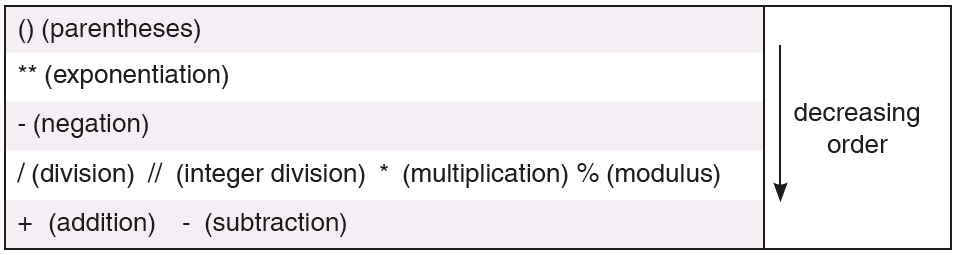
\includegraphics{3.png}

    \begin{center}\rule{0.5\linewidth}{\linethickness}\end{center}

\subsection{ Relational Operators }\label{relational-operators}

\begin{itemize}
\tightlist
\item
  Used for comparing two expressions and yield True or False.
\item
  The arithmetic operators have higher precedence than the relational
  operators.
\end{itemize}

    \begin{Verbatim}[commandchars=\\\{\}]
{\color{incolor}In [{\color{incolor} }]:} \PY{n+nb}{print}\PY{p}{(}\PY{l+s+s2}{\PYZdq{}}\PY{l+s+s2}{23 \PYZlt{} 25  :}\PY{l+s+s2}{\PYZdq{}}\PY{p}{,} \PY{l+m+mi}{23} \PY{o}{\PYZlt{}} \PY{l+m+mi}{25}\PY{p}{)}           \PY{c+c1}{\PYZsh{}less than}
        \PY{n+nb}{print}\PY{p}{(}\PY{l+s+s2}{\PYZdq{}}\PY{l+s+s2}{23 \PYZgt{} 25  :}\PY{l+s+s2}{\PYZdq{}}\PY{p}{,} \PY{l+m+mi}{23} \PY{o}{\PYZgt{}} \PY{l+m+mi}{25}\PY{p}{)}           \PY{c+c1}{\PYZsh{}greater than}
        \PY{n+nb}{print}\PY{p}{(}\PY{l+s+s2}{\PYZdq{}}\PY{l+s+s2}{23 \PYZlt{}= 23 :}\PY{l+s+s2}{\PYZdq{}}\PY{p}{,} \PY{l+m+mi}{23} \PY{o}{\PYZlt{}}\PY{o}{=} \PY{l+m+mi}{23}\PY{p}{)}          \PY{c+c1}{\PYZsh{}less than or equal to}
        \PY{n+nb}{print}\PY{p}{(}\PY{l+s+s2}{\PYZdq{}}\PY{l+s+s2}{23 \PYZhy{} 2.5 \PYZgt{}= 5 * 4 :}\PY{l+s+s2}{\PYZdq{}}\PY{p}{,} \PY{l+m+mi}{23} \PY{o}{\PYZhy{}} \PY{l+m+mf}{2.5} \PY{o}{\PYZgt{}}\PY{o}{=} \PY{l+m+mi}{5} \PY{o}{*} \PY{l+m+mi}{4}\PY{p}{)} \PY{c+c1}{\PYZsh{}greater than or equal to}
        \PY{n+nb}{print}\PY{p}{(}\PY{l+s+s2}{\PYZdq{}}\PY{l+s+s2}{23 == 25 :}\PY{l+s+s2}{\PYZdq{}}\PY{p}{,} \PY{l+m+mi}{23} \PY{o}{==} \PY{l+m+mi}{25}\PY{p}{)}          \PY{c+c1}{\PYZsh{}equal to}
        \PY{n+nb}{print}\PY{p}{(}\PY{l+s+s2}{\PYZdq{}}\PY{l+s+s2}{23 != 25 :}\PY{l+s+s2}{\PYZdq{}}\PY{p}{,} \PY{l+m+mi}{23} \PY{o}{!=} \PY{l+m+mi}{25}\PY{p}{)}          \PY{c+c1}{\PYZsh{}not equal to}
\end{Verbatim}


    \begin{itemize}
\tightlist
\item
  When the relational operators are applied to strings, strings are
  compared left to right, character by character, based on their ASCII
  codes, also called ASCII values.
\end{itemize}

    \begin{Verbatim}[commandchars=\\\{\}]
{\color{incolor}In [{\color{incolor}12}]:} \PY{n+nb}{print}\PY{p}{(}\PY{l+s+s2}{\PYZdq{}}\PY{l+s+s2}{\PYZsq{}}\PY{l+s+s2}{hello}\PY{l+s+s2}{\PYZsq{}}\PY{l+s+s2}{ \PYZlt{} }\PY{l+s+s2}{\PYZsq{}}\PY{l+s+s2}{Hello}\PY{l+s+s2}{\PYZsq{}}\PY{l+s+s2}{ :}\PY{l+s+s2}{\PYZdq{}}\PY{p}{,} \PY{l+s+s1}{\PYZsq{}}\PY{l+s+s1}{hello}\PY{l+s+s1}{\PYZsq{}} \PY{o}{\PYZlt{}} \PY{l+s+s1}{\PYZsq{}}\PY{l+s+s1}{Hello}\PY{l+s+s1}{\PYZsq{}}\PY{p}{)} 
         \PY{n+nb}{print}\PY{p}{(}\PY{l+s+s2}{\PYZdq{}}\PY{l+s+s2}{\PYZsq{}}\PY{l+s+s2}{hi}\PY{l+s+s2}{\PYZsq{}}\PY{l+s+s2}{ \PYZgt{} }\PY{l+s+s2}{\PYZsq{}}\PY{l+s+s2}{hello}\PY{l+s+s2}{\PYZsq{}}\PY{l+s+s2}{    :}\PY{l+s+s2}{\PYZdq{}}\PY{p}{,} \PY{l+s+s1}{\PYZsq{}}\PY{l+s+s1}{hi}\PY{l+s+s1}{\PYZsq{}} \PY{o}{\PYZgt{}} \PY{l+s+s1}{\PYZsq{}}\PY{l+s+s1}{hello}\PY{l+s+s1}{\PYZsq{}}\PY{p}{)} 
\end{Verbatim}


    \begin{Verbatim}[commandchars=\\\{\}]
'hello' < 'Hello' : False
'hi' > 'hello'    : True

    \end{Verbatim}

    \begin{center}\rule{0.5\linewidth}{\linethickness}\end{center}

\subsection{ Logical Operators }\label{logical-operators}

\begin{itemize}
\tightlist
\item
  The logical operators not, and, and or are applied to logical operands
  True and False, also called Boolean values, and yield either True or
  False.
\item
  As compared to relational and arithmetic operators, logical operators
  have the least precedence level.
\end{itemize}

    \begin{Verbatim}[commandchars=\\\{\}]
{\color{incolor}In [{\color{incolor} }]:} \PY{n+nb}{print}\PY{p}{(}\PY{l+s+s2}{\PYZdq{}}\PY{l+s+s2}{not True \PYZlt{} 25      :}\PY{l+s+s2}{\PYZdq{}}\PY{p}{,} \PY{o+ow}{not} \PY{k+kc}{True}\PY{p}{)}              \PY{c+c1}{\PYZsh{}not operator}
        \PY{n+nb}{print}\PY{p}{(}\PY{l+s+s2}{\PYZdq{}}\PY{l+s+s2}{10 \PYZlt{} 25 and 5 \PYZgt{} 6  :}\PY{l+s+s2}{\PYZdq{}}\PY{p}{,} \PY{l+m+mi}{10} \PY{o}{\PYZlt{}} \PY{l+m+mi}{25} \PY{o+ow}{and} \PY{l+m+mi}{5} \PY{o}{\PYZgt{}} \PY{l+m+mi}{6}\PY{p}{)} \PY{c+c1}{\PYZsh{}and operator}
        \PY{n+nb}{print}\PY{p}{(}\PY{l+s+s2}{\PYZdq{}}\PY{l+s+s2}{10 \PYZlt{} 25 or 5 \PYZgt{} 6   :}\PY{l+s+s2}{\PYZdq{}}\PY{p}{,} \PY{l+m+mi}{10} \PY{o}{\PYZlt{}} \PY{l+m+mi}{25} \PY{o+ow}{or} \PY{l+m+mi}{5} \PY{o}{\PYZgt{}} \PY{l+m+mi}{6}\PY{p}{)}   \PY{c+c1}{\PYZsh{}or operator}
\end{Verbatim}


    \subsubsection{ Precedence of Logical Operators
}\label{precedence-of-logical-operators}

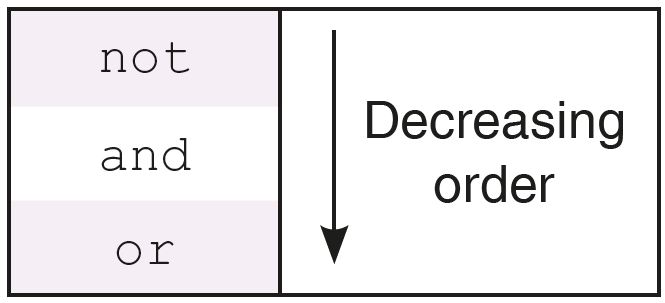
\includegraphics{4.png}

    \begin{center}\rule{0.5\linewidth}{\linethickness}\end{center}

\subsection{ Python Keywords }\label{python-keywords}

\begin{itemize}
\tightlist
\item
  Reserved words that are already defined by the Python for specific
  uses.
\end{itemize}

    \begin{Verbatim}[commandchars=\\\{\}]
{\color{incolor}In [{\color{incolor} }]:} \PY{k+kn}{import} \PY{n+nn}{keyword}
        \PY{n+nb}{print}\PY{p}{(}\PY{n}{keyword}\PY{o}{.}\PY{n}{kwlist}\PY{p}{)}
\end{Verbatim}


    {[}'False', 'None', 'True', 'and', 'as', 'assert', 'break',
'class','continue', 'def', 'del', 'elif', 'else', 'except', 'finally',
'for', 'from', 'global', 'if', 'import', 'in', 'is',
'lambda','nonlocal', 'not', 'or', 'pass', 'raise', 'return', 'try',
'while', 'with', 'yield'{]}

    \begin{center}\rule{0.5\linewidth}{\linethickness}\end{center}

\subsection{ Functions }\label{functions}

\begin{itemize}
\tightlist
\item
  Functions provide a systematic way of problem solving by dividing the
  given problem into several sub-problems, finding their individual
  solutions, and integrating the solutions of individual problems to
  solve the original problem.
\item
  This approach to problem solving is called stepwise refinement method
  or modular approach.
\end{itemize}

    \subsection{ Built-in Functions }\label{built-in-functions}

\begin{itemize}
\tightlist
\item
  Predefined functions that are already available in Python.
\end{itemize}

    \subsubsection{ Type Conversion: int, float, str functions
}\label{type-conversion-int-float-str-functions}

    \begin{Verbatim}[commandchars=\\\{\}]
{\color{incolor}In [{\color{incolor}13}]:} \PY{n+nb}{str}\PY{p}{(}\PY{l+m+mi}{123}\PY{p}{)}
\end{Verbatim}


\begin{Verbatim}[commandchars=\\\{\}]
{\color{outcolor}Out[{\color{outcolor}13}]:} '123'
\end{Verbatim}
            
    \begin{Verbatim}[commandchars=\\\{\}]
{\color{incolor}In [{\color{incolor}14}]:} \PY{n+nb}{int}\PY{p}{(}\PY{l+s+s1}{\PYZsq{}}\PY{l+s+s1}{234}\PY{l+s+s1}{\PYZsq{}}\PY{p}{)}
\end{Verbatim}


\begin{Verbatim}[commandchars=\\\{\}]
{\color{outcolor}Out[{\color{outcolor}14}]:} 234
\end{Verbatim}
            
    \begin{Verbatim}[commandchars=\\\{\}]
{\color{incolor}In [{\color{incolor}15}]:} \PY{n+nb}{int}\PY{p}{(}\PY{l+m+mf}{234.8}\PY{p}{)}
\end{Verbatim}


\begin{Verbatim}[commandchars=\\\{\}]
{\color{outcolor}Out[{\color{outcolor}15}]:} 234
\end{Verbatim}
            
    \subsubsection{ input function }\label{input-function}

\begin{itemize}
\tightlist
\item
  Enables us to accept an input string from the user without evaluating
  its value.
\item
  The function input continues to read input text from the user until it
  encounters a newline.
\end{itemize}

    \begin{Verbatim}[commandchars=\\\{\}]
{\color{incolor}In [{\color{incolor}16}]:} \PY{n}{name} \PY{o}{=} \PY{n+nb}{input}\PY{p}{(}\PY{l+s+s1}{\PYZsq{}}\PY{l+s+s1}{Enter a name: }\PY{l+s+s1}{\PYZsq{}}\PY{p}{)}
         \PY{n+nb}{print}\PY{p}{(}\PY{l+s+s1}{\PYZsq{}}\PY{l+s+s1}{Welcome}\PY{l+s+s1}{\PYZsq{}}\PY{p}{,} \PY{n}{name}\PY{p}{)}
\end{Verbatim}


    \begin{Verbatim}[commandchars=\\\{\}]
Enter a name: Suresh
Welcome Suresh

    \end{Verbatim}

    \begin{Verbatim}[commandchars=\\\{\}]
{\color{incolor}In [{\color{incolor}21}]:} \PY{n}{costPrice} \PY{o}{=} \PY{n+nb}{int}\PY{p}{(}\PY{n+nb}{input}\PY{p}{(}\PY{l+s+s1}{\PYZsq{}}\PY{l+s+s1}{Enter cost price: }\PY{l+s+s1}{\PYZsq{}}\PY{p}{)}\PY{p}{)}
         \PY{n}{profit} \PY{o}{=} \PY{n+nb}{int}\PY{p}{(}\PY{n+nb}{input}\PY{p}{(}\PY{l+s+s1}{\PYZsq{}}\PY{l+s+s1}{Enter profit: }\PY{l+s+s1}{\PYZsq{}}\PY{p}{)}\PY{p}{)}
         \PY{n}{sellingPrice} \PY{o}{=} \PY{n}{costPrice} \PY{o}{+} \PY{n}{profit}
         \PY{n+nb}{print}\PY{p}{(}\PY{l+s+s1}{\PYZsq{}}\PY{l+s+s1}{Selling Price: }\PY{l+s+s1}{\PYZsq{}}\PY{p}{,} \PY{n}{sellingPrice}\PY{p}{)}
\end{Verbatim}


    \begin{Verbatim}[commandchars=\\\{\}]
Enter cost price: 50
Enter profit: 12
Selling Price:  62

    \end{Verbatim}

    \subsubsection{ eval function }\label{eval-function}

\begin{itemize}
\tightlist
\item
  Used to evaluate the value of a string.
\end{itemize}

    \begin{Verbatim}[commandchars=\\\{\}]
{\color{incolor}In [{\color{incolor}22}]:} \PY{n}{a} \PY{o}{=} \PY{n+nb}{eval}\PY{p}{(}\PY{l+s+s1}{\PYZsq{}}\PY{l+s+s1}{15+10}\PY{l+s+s1}{\PYZsq{}}\PY{p}{)}
         \PY{n+nb}{print}\PY{p}{(}\PY{n}{a}\PY{p}{)}
\end{Verbatim}


    \begin{Verbatim}[commandchars=\\\{\}]
25

    \end{Verbatim}

    \subsubsection{ min and max functions }\label{min-and-max-functions}

\begin{itemize}
\tightlist
\item
  Used to find maximum and minimum value respectively out of several
  values.
\end{itemize}

    \begin{Verbatim}[commandchars=\\\{\}]
{\color{incolor}In [{\color{incolor}23}]:} \PY{n}{a} \PY{o}{=} \PY{n+nb}{max}\PY{p}{(}\PY{l+m+mi}{59}\PY{p}{,} \PY{l+m+mi}{80}\PY{p}{,} \PY{l+m+mf}{95.6}\PY{p}{,} \PY{l+m+mf}{95.2}\PY{p}{)}
         \PY{n}{b} \PY{o}{=} \PY{n+nb}{min}\PY{p}{(}\PY{l+s+s1}{\PYZsq{}}\PY{l+s+s1}{hello}\PY{l+s+s1}{\PYZsq{}}\PY{p}{,} \PY{l+s+s1}{\PYZsq{}}\PY{l+s+s1}{how}\PY{l+s+s1}{\PYZsq{}}\PY{p}{,} \PY{l+s+s1}{\PYZsq{}}\PY{l+s+s1}{are}\PY{l+s+s1}{\PYZsq{}}\PY{p}{,} \PY{l+s+s1}{\PYZsq{}}\PY{l+s+s1}{you}\PY{l+s+s1}{\PYZsq{}}\PY{p}{,} \PY{l+s+s1}{\PYZsq{}}\PY{l+s+s1}{Sir}\PY{l+s+s1}{\PYZsq{}}\PY{p}{)}
         \PY{n+nb}{print}\PY{p}{(}\PY{l+s+s2}{\PYZdq{}}\PY{l+s+s2}{Minimum Value}\PY{l+s+s2}{\PYZdq{}}\PY{p}{,} \PY{n}{a}\PY{p}{)}
         \PY{n+nb}{print}\PY{p}{(}\PY{l+s+s2}{\PYZdq{}}\PY{l+s+s2}{Maximum Value}\PY{l+s+s2}{\PYZdq{}}\PY{p}{,} \PY{n}{b}\PY{p}{)}
\end{Verbatim}


    \begin{Verbatim}[commandchars=\\\{\}]
Minimum Value 95.6
Maximum Value Sir

    \end{Verbatim}

    \subsubsection{ Functions from math module
}\label{functions-from-math-module}

\begin{itemize}
\tightlist
\item
  Used to find maximum and minimum value respectively out of several
  values.
\end{itemize}

    \begin{Verbatim}[commandchars=\\\{\}]
{\color{incolor}In [{\color{incolor}25}]:} \PY{k+kn}{import} \PY{n+nn}{math}
         \PY{n+nb}{print}\PY{p}{(}\PY{l+s+s2}{\PYZdq{}}\PY{l+s+s2}{math.ceil(3.4)  :}\PY{l+s+s2}{\PYZdq{}}\PY{p}{,} \PY{n}{math}\PY{o}{.}\PY{n}{ceil}\PY{p}{(}\PY{l+m+mf}{3.4}\PY{p}{)}\PY{p}{)}
         \PY{n+nb}{print}\PY{p}{(}\PY{l+s+s2}{\PYZdq{}}\PY{l+s+s2}{math.pow(3, 3)  :}\PY{l+s+s2}{\PYZdq{}}\PY{p}{,} \PY{n}{math}\PY{o}{.}\PY{n}{pow}\PY{p}{(}\PY{l+m+mi}{3}\PY{p}{,} \PY{l+m+mi}{3}\PY{p}{)}\PY{p}{)}
         \PY{n+nb}{print}\PY{p}{(}\PY{l+s+s2}{\PYZdq{}}\PY{l+s+s2}{math.sqrt(65)   :}\PY{l+s+s2}{\PYZdq{}}\PY{p}{,} \PY{n}{math}\PY{o}{.}\PY{n}{sqrt}\PY{p}{(}\PY{l+m+mi}{65}\PY{p}{)}\PY{p}{)}
         \PY{n+nb}{print}\PY{p}{(}\PY{l+s+s2}{\PYZdq{}}\PY{l+s+s2}{math.sqrt(65)   :}\PY{l+s+s2}{\PYZdq{}}\PY{p}{,} \PY{n+nb}{round}\PY{p}{(}\PY{n}{math}\PY{o}{.}\PY{n}{sqrt}\PY{p}{(}\PY{l+m+mi}{65}\PY{p}{)}\PY{p}{,}\PY{l+m+mi}{2}\PY{p}{)}\PY{p}{)}
         \PY{n+nb}{print}\PY{p}{(}\PY{l+s+s2}{\PYZdq{}}\PY{l+s+s2}{math.log10(100) :}\PY{l+s+s2}{\PYZdq{}}\PY{p}{,} \PY{n}{math}\PY{o}{.}\PY{n}{log10}\PY{p}{(}\PY{l+m+mi}{100}\PY{p}{)}\PY{p}{)}
\end{Verbatim}


    \begin{Verbatim}[commandchars=\\\{\}]
math.ceil(3.4)  : 4
math.pow(3, 3)  : 27.0
math.sqrt(65)   : 8.06225774829855
math.sqrt(65)   : 8.06
math.log10(100) : 2.0

    \end{Verbatim}

    \subsubsection{ help function }\label{help-function}

\begin{itemize}
\tightlist
\item
  Used to know the purpose of a function and how it is used.
\end{itemize}

    \begin{Verbatim}[commandchars=\\\{\}]
{\color{incolor}In [{\color{incolor}26}]:} \PY{k+kn}{import} \PY{n+nn}{math}
         \PY{n+nb}{print}\PY{p}{(}\PY{n}{help}\PY{p}{(}\PY{n}{math}\PY{o}{.}\PY{n}{cos}\PY{p}{)}\PY{p}{)}
\end{Verbatim}


    \begin{Verbatim}[commandchars=\\\{\}]
Help on built-in function cos in module math:

cos({\ldots})
    cos(x)
    
    Return the cosine of x (measured in radians).

None

    \end{Verbatim}

    \subsection{ Function Definition and Call
}\label{function-definition-and-call}

    \begin{quote}
The \textbf{syntax} for a function definition is as follows:
\end{quote}

\begin{verbatim}
def function_name ( comma_separated_list_of_parameters):
    statements
\end{verbatim}

Note: Statements below \textbf{def} begin with four spaces. This is
called \textbf{indentation}. It is a requirement of Python that the code
following a colon must be indented.

    \begin{Verbatim}[commandchars=\\\{\}]
{\color{incolor}In [{\color{incolor}28}]:} \PY{k}{def} \PY{n+nf}{triangle}\PY{p}{(}\PY{p}{)}\PY{p}{:}
             \PY{l+s+sd}{\PYZsq{}\PYZsq{}\PYZsq{}}
         \PY{l+s+sd}{    Objective: To print a right angled triangle.}
         \PY{l+s+sd}{    Input Parameter: None}
         \PY{l+s+sd}{    Return Value: None}
         \PY{l+s+sd}{    \PYZsq{}\PYZsq{}\PYZsq{}}
             \PY{l+s+sd}{\PYZsq{}\PYZsq{}\PYZsq{}}
         \PY{l+s+sd}{    Approach: To use a print statement for each line of output}
         \PY{l+s+sd}{    \PYZsq{}\PYZsq{}\PYZsq{}}
             \PY{n+nb}{print}\PY{p}{(}\PY{l+s+s1}{\PYZsq{}}\PY{l+s+s1}{*}\PY{l+s+s1}{\PYZsq{}}\PY{p}{)}
             \PY{n+nb}{print}\PY{p}{(}\PY{l+s+s1}{\PYZsq{}}\PY{l+s+s1}{* *}\PY{l+s+s1}{\PYZsq{}}\PY{p}{)}
             \PY{n+nb}{print}\PY{p}{(}\PY{l+s+s1}{\PYZsq{}}\PY{l+s+s1}{* * *}\PY{l+s+s1}{\PYZsq{}}\PY{p}{)}
             \PY{n+nb}{print}\PY{p}{(}\PY{l+s+s1}{\PYZsq{}}\PY{l+s+s1}{* * * *}\PY{l+s+s1}{\PYZsq{}}\PY{p}{)}
\end{Verbatim}


    \paragraph{Invoking the function}\label{invoking-the-function}

    \begin{Verbatim}[commandchars=\\\{\}]
{\color{incolor}In [{\color{incolor}29}]:} \PY{n}{triangle}\PY{p}{(}\PY{p}{)}
\end{Verbatim}


    \begin{Verbatim}[commandchars=\\\{\}]
*
* *
* * *
* * * *

    \end{Verbatim}

    \subsubsection{ Computing Area of the Rectangle
}\label{computing-area-of-the-rectangle}

    \begin{Verbatim}[commandchars=\\\{\}]
{\color{incolor}In [{\color{incolor}30}]:} \PY{k}{def} \PY{n+nf}{areaRectangle}\PY{p}{(}\PY{n}{length}\PY{p}{,} \PY{n}{breadth}\PY{p}{)}\PY{p}{:}
             \PY{l+s+sd}{\PYZsq{}\PYZsq{}\PYZsq{}}
         \PY{l+s+sd}{    Objective: To compute the area of rectangle}
         \PY{l+s+sd}{    Input Parameters: length, breadth – numeric value}
         \PY{l+s+sd}{    Return Value: area \PYZhy{} numeric value}
         \PY{l+s+sd}{    \PYZsq{}\PYZsq{}\PYZsq{}}
             \PY{n}{area} \PY{o}{=} \PY{n}{length} \PY{o}{*} \PY{n}{breadth}
             \PY{k}{return} \PY{n}{area}
\end{Verbatim}


    \begin{Verbatim}[commandchars=\\\{\}]
{\color{incolor}In [{\color{incolor}33}]:} \PY{n}{areaRectangle}\PY{p}{(}\PY{l+m+mi}{7}\PY{p}{,}\PY{l+m+mi}{5}\PY{p}{)}
\end{Verbatim}


\begin{Verbatim}[commandchars=\\\{\}]
{\color{outcolor}Out[{\color{outcolor}33}]:} 35
\end{Verbatim}
            
    \begin{Verbatim}[commandchars=\\\{\}]
{\color{incolor}In [{\color{incolor}34}]:} \PY{n}{help}\PY{p}{(}\PY{n}{areaRectangle}\PY{p}{)}
\end{Verbatim}


    \begin{Verbatim}[commandchars=\\\{\}]
Help on function areaRectangle in module \_\_main\_\_:

areaRectangle(length, breadth)
    Objective: To compute the area of rectangle
    Input Parameters: length, breadth – numeric value
    Return Value: area - numeric value


    \end{Verbatim}

    \begin{Verbatim}[commandchars=\\\{\}]
{\color{incolor}In [{\color{incolor}43}]:} \PY{k}{def} \PY{n+nf}{areaRectangle}\PY{p}{(}\PY{n}{length}\PY{p}{,} \PY{n}{breadth}\PY{o}{=}\PY{l+m+mi}{1}\PY{p}{)}\PY{p}{:}
             \PY{l+s+sd}{\PYZsq{}\PYZsq{}\PYZsq{}}
         \PY{l+s+sd}{    Objective: To compute the area of rectangle}
         \PY{l+s+sd}{    Input Parameters: length, breadth \PYZhy{} numeric value}
         \PY{l+s+sd}{    Return Value: area \PYZhy{} numeric value}
         \PY{l+s+sd}{    \PYZsq{}\PYZsq{}\PYZsq{}}
             \PY{n}{area} \PY{o}{=} \PY{n}{length} \PY{o}{*} \PY{n}{breadth}
             \PY{k}{return} \PY{n}{area}
         
         \PY{k}{def} \PY{n+nf}{main}\PY{p}{(}\PY{p}{)}\PY{p}{:}
             \PY{l+s+sd}{\PYZsq{}\PYZsq{}\PYZsq{}}
         \PY{l+s+sd}{    Objective: To compute the area of rectangle based on user input}
         \PY{l+s+sd}{    Input Parameter: None}
         \PY{l+s+sd}{    Return Value: None}
         \PY{l+s+sd}{    \PYZsq{}\PYZsq{}\PYZsq{}}
             \PY{n+nb}{print}\PY{p}{(}\PY{l+s+s1}{\PYZsq{}}\PY{l+s+s1}{Enter the following values for rectangle:}\PY{l+s+s1}{\PYZsq{}}\PY{p}{)}
             \PY{n}{lengthRect} \PY{o}{=} \PY{n+nb}{int}\PY{p}{(}\PY{n+nb}{input}\PY{p}{(}\PY{l+s+s1}{\PYZsq{}}\PY{l+s+s1}{Length : integer value: }\PY{l+s+s1}{\PYZsq{}}\PY{p}{)}\PY{p}{)}
             \PY{n}{breadthRect} \PY{o}{=} \PY{n+nb}{int}\PY{p}{(}\PY{n+nb}{input}\PY{p}{(}\PY{l+s+s1}{\PYZsq{}}\PY{l+s+s1}{Breadth : integer value: }\PY{l+s+s1}{\PYZsq{}}\PY{p}{)}\PY{p}{)}
             \PY{n}{areaRect} \PY{o}{=} \PY{n}{areaRectangle}\PY{p}{(}\PY{n}{lengthRect}\PY{p}{,} \PY{n}{breadthRect}\PY{p}{)}
             \PY{n+nb}{print}\PY{p}{(}\PY{l+s+s1}{\PYZsq{}}\PY{l+s+s1}{Area of rectangle is}\PY{l+s+s1}{\PYZsq{}}\PY{p}{,} \PY{n}{areaRect}\PY{p}{)}
             
         \PY{k}{if} \PY{n+nv+vm}{\PYZus{}\PYZus{}name\PYZus{}\PYZus{}} \PY{o}{==} \PY{l+s+s1}{\PYZsq{}}\PY{l+s+s1}{\PYZus{}\PYZus{}main\PYZus{}\PYZus{}}\PY{l+s+s1}{\PYZsq{}}\PY{p}{:}
             \PY{n}{main}\PY{p}{(}\PY{p}{)}
\end{Verbatim}


    \begin{Verbatim}[commandchars=\\\{\}]
Enter the following values for rectangle:
Length : integer value: 7
Breadth : integer value: 5
Area of rectangle is 35

    \end{Verbatim}

    \begin{center}\rule{0.5\linewidth}{\linethickness}\end{center}

\subsection{ Control Structures }\label{control-structures}

\begin{itemize}
\tightlist
\item
  Needed for non-sequential and repetitive execution of instructions.
\end{itemize}

    \subsection{ if Conditional Statement }\label{if-conditional-statement}

\begin{itemize}
\item
  Used to execute a certain sequence of statements depending upon
  fulfilment of a particular condition \textgreater{} The general form
  of \textbf{if-elif-else} statement is as follows:

  if \textless{} condition1 \textgreater{}: \textless{} Sequence S1 of
  statements to be executed \textgreater{} elif \textless{} condition2
  \textgreater{}: \textless{} Sequence S2 of statements to be executed
  \textgreater{} elif \textless{} condition3 \textgreater{}: \textless{}
  Sequence S3 of statements to be executed \textgreater{} ...

  else: \textless{} Sequence Sn of statements to be executed
  \textgreater{}
\end{itemize}

    \subsubsection{Problem: Grade assignment on the basis of marks
obtained}\label{problem-grade-assignment-on-the-basis-of-marks-obtained}

    \begin{Verbatim}[commandchars=\\\{\}]
{\color{incolor}In [{\color{incolor}44}]:} \PY{k}{def} \PY{n+nf}{assignGrade}\PY{p}{(}\PY{n}{marks}\PY{p}{)}\PY{p}{:}
             \PY{l+s+sd}{\PYZsq{}\PYZsq{}\PYZsq{}}
         \PY{l+s+sd}{    Objective: To assign grade on the basis of marks obtained}
         \PY{l+s+sd}{    Input Parameter: marks – numeric value}
         \PY{l+s+sd}{    Return Value: grade \PYZhy{} string}
         \PY{l+s+sd}{    \PYZsq{}\PYZsq{}\PYZsq{}}
             \PY{k}{assert} \PY{n}{marks} \PY{o}{\PYZgt{}}\PY{o}{=} \PY{l+m+mi}{0} \PY{o+ow}{and} \PY{n}{marks} \PY{o}{\PYZlt{}}\PY{o}{=} \PY{l+m+mi}{100}
             \PY{k}{if} \PY{n}{marks} \PY{o}{\PYZgt{}}\PY{o}{=} \PY{l+m+mi}{90}\PY{p}{:}
                 \PY{n}{grade} \PY{o}{=} \PY{l+s+s1}{\PYZsq{}}\PY{l+s+s1}{A}\PY{l+s+s1}{\PYZsq{}}
             \PY{k}{elif} \PY{n}{marks} \PY{o}{\PYZgt{}}\PY{o}{=} \PY{l+m+mi}{70}\PY{p}{:}
                 \PY{n}{grade} \PY{o}{=} \PY{l+s+s1}{\PYZsq{}}\PY{l+s+s1}{B}\PY{l+s+s1}{\PYZsq{}}
             \PY{k}{elif} \PY{n}{marks} \PY{o}{\PYZgt{}}\PY{o}{=} \PY{l+m+mi}{50}\PY{p}{:}
                 \PY{n}{grade} \PY{o}{=} \PY{l+s+s1}{\PYZsq{}}\PY{l+s+s1}{C}\PY{l+s+s1}{\PYZsq{}}
             \PY{k}{elif} \PY{n}{marks} \PY{o}{\PYZgt{}}\PY{o}{=} \PY{l+m+mi}{40}\PY{p}{:}
                 \PY{n}{grade} \PY{o}{=} \PY{l+s+s1}{\PYZsq{}}\PY{l+s+s1}{D}\PY{l+s+s1}{\PYZsq{}}
             \PY{k}{else}\PY{p}{:}
                 \PY{n}{grade} \PY{o}{=} \PY{l+s+s1}{\PYZsq{}}\PY{l+s+s1}{F}\PY{l+s+s1}{\PYZsq{}}
             \PY{k}{return} \PY{n}{grade}
         
         \PY{k}{def} \PY{n+nf}{main}\PY{p}{(}\PY{p}{)}\PY{p}{:}
             \PY{l+s+sd}{\PYZsq{}\PYZsq{}\PYZsq{}}
         \PY{l+s+sd}{    Objective: To assign grade on the basis of input marks}
         \PY{l+s+sd}{    Input Parameter: None}
         \PY{l+s+sd}{    Return Value: None}
         \PY{l+s+sd}{    \PYZsq{}\PYZsq{}\PYZsq{}}
             \PY{n}{marks} \PY{o}{=} \PY{n+nb}{float}\PY{p}{(}\PY{n+nb}{input}\PY{p}{(}\PY{l+s+s1}{\PYZsq{}}\PY{l+s+s1}{Enter your marks: }\PY{l+s+s1}{\PYZsq{}}\PY{p}{)}\PY{p}{)}
             \PY{n+nb}{print}\PY{p}{(}\PY{l+s+s1}{\PYZsq{}}\PY{l+s+s1}{Marks:}\PY{l+s+s1}{\PYZsq{}}\PY{p}{,} \PY{n}{marks}\PY{p}{,} \PY{l+s+s1}{\PYZsq{}}\PY{l+s+se}{\PYZbs{}n}\PY{l+s+s1}{Grade:}\PY{l+s+s1}{\PYZsq{}}\PY{p}{,} \PY{n}{assignGrade}\PY{p}{(}\PY{n}{marks}\PY{p}{)}\PY{p}{)}
         
         \PY{k}{if} \PY{n+nv+vm}{\PYZus{}\PYZus{}name\PYZus{}\PYZus{}} \PY{o}{==} \PY{l+s+s1}{\PYZsq{}}\PY{l+s+s1}{\PYZus{}\PYZus{}main\PYZus{}\PYZus{}}\PY{l+s+s1}{\PYZsq{}}\PY{p}{:}
             \PY{n}{main}\PY{p}{(}\PY{p}{)}
\end{Verbatim}


    \begin{Verbatim}[commandchars=\\\{\}]
Enter your marks: 89
Marks: 89.0 
Grade: B

    \end{Verbatim}

    \subsection{ for Statement }\label{for-statement}

\begin{itemize}
\item
  It is used when we want to execute a sequence of statements (indented
  to the right of keyword for) a fixed number of times. \textgreater{}
  Syntax of \textbf{for} statement is as follows:

  for variable in sequence: 
\end{itemize}

    \begin{Verbatim}[commandchars=\\\{\}]
{\color{incolor}In [{\color{incolor}38}]:} \PY{k}{for} \PY{n}{letter} \PY{o+ow}{in} \PY{l+s+s2}{\PYZdq{}}\PY{l+s+s2}{hello}\PY{l+s+s2}{\PYZdq{}}\PY{p}{:}
             \PY{n+nb}{print}\PY{p}{(}\PY{n}{letter}\PY{p}{)}
\end{Verbatim}


    \begin{Verbatim}[commandchars=\\\{\}]
h
e
l
l
o

    \end{Verbatim}

    \subsubsection{ Generating sequence of numbers using range
function}\label{generating-sequence-of-numbers-using-range-function}

\begin{quote}
Syntax:
\end{quote}

\begin{verbatim}
range(start, end, increment)
\end{verbatim}

    The function call \textbf{range(1,n + 1)} produces a sequence of numbers
from 1 to n

    \begin{Verbatim}[commandchars=\\\{\}]
{\color{incolor}In [{\color{incolor} }]:} \PY{n}{start} \PY{o}{=} \PY{l+m+mi}{1}
        \PY{n}{limit} \PY{o}{=} \PY{l+m+mi}{11}
        \PY{k}{for} \PY{n}{num} \PY{o+ow}{in} \PY{n+nb}{range}\PY{p}{(}\PY{n}{start}\PY{p}{,} \PY{n}{limit}\PY{p}{)}\PY{p}{:}
            \PY{n+nb}{print}\PY{p}{(}\PY{n}{num}\PY{p}{)}
\end{Verbatim}


    \begin{Verbatim}[commandchars=\\\{\}]
{\color{incolor}In [{\color{incolor} }]:} \PY{n}{start} \PY{o}{=} \PY{l+m+mi}{1}
        \PY{n}{limit} \PY{o}{=} \PY{l+m+mi}{11}
        \PY{n}{step} \PY{o}{=} \PY{l+m+mi}{2}
        \PY{k}{for} \PY{n}{num} \PY{o+ow}{in} \PY{n+nb}{range}\PY{p}{(}\PY{n}{start}\PY{p}{,} \PY{n}{limit}\PY{p}{,} \PY{n}{step}\PY{p}{)}\PY{p}{:}
            \PY{n+nb}{print}\PY{p}{(}\PY{n}{num}\PY{p}{)}
\end{Verbatim}


    \begin{Verbatim}[commandchars=\\\{\}]
{\color{incolor}In [{\color{incolor} }]:} \PY{n}{start} \PY{o}{=} \PY{l+m+mi}{30}
        \PY{n}{limit} \PY{o}{=} \PY{o}{\PYZhy{}}\PY{l+m+mi}{4}
        \PY{n}{step} \PY{o}{=} \PY{o}{\PYZhy{}}\PY{l+m+mi}{3}
        \PY{k}{for} \PY{n}{num} \PY{o+ow}{in} \PY{n+nb}{range}\PY{p}{(}\PY{n}{start}\PY{p}{,} \PY{n}{limit}\PY{p}{,} \PY{n}{step}\PY{p}{)}\PY{p}{:}
            \PY{n+nb}{print}\PY{p}{(}\PY{n}{num}\PY{p}{)}
\end{Verbatim}


    \begin{Verbatim}[commandchars=\\\{\}]
{\color{incolor}In [{\color{incolor} }]:} \PY{n}{limit} \PY{o}{=} \PY{l+m+mi}{5}
        \PY{k}{for} \PY{n}{num} \PY{o+ow}{in} \PY{n+nb}{range}\PY{p}{(}\PY{n}{limit}\PY{p}{)}\PY{p}{:}
            \PY{n+nb}{print}\PY{p}{(}\PY{n}{num}\PY{p}{)}
\end{Verbatim}


    \subsubsection{ Problem: Printing a Triangle
}\label{problem-printing-a-triangle}

    \begin{Verbatim}[commandchars=\\\{\}]
{\color{incolor}In [{\color{incolor}1}]:} \PY{k}{def} \PY{n+nf}{rightTriangle}\PY{p}{(}\PY{n}{rows}\PY{p}{)}\PY{p}{:}
            \PY{l+s+sd}{\PYZsq{}\PYZsq{}\PYZsq{}}
        \PY{l+s+sd}{    Objective: To print a triangle comprising of asterisks}
        \PY{l+s+sd}{    Input Parameter: rows \PYZhy{} numeric}
        \PY{l+s+sd}{    Return Value: None}
        \PY{l+s+sd}{    \PYZsq{}\PYZsq{}\PYZsq{}}
            \PY{k}{for} \PY{n}{i} \PY{o+ow}{in} \PY{n+nb}{range}\PY{p}{(}\PY{l+m+mi}{1}\PY{p}{,} \PY{n}{rows} \PY{o}{+} \PY{l+m+mi}{1}\PY{p}{)}\PY{p}{:}
                \PY{n+nb}{print}\PY{p}{(}\PY{l+s+s1}{\PYZsq{}}\PY{l+s+s1}{*}\PY{l+s+s1}{\PYZsq{}} \PY{o}{*} \PY{n}{i}\PY{p}{)}
            
        \PY{k}{def} \PY{n+nf}{main}\PY{p}{(}\PY{p}{)}\PY{p}{:}
            \PY{l+s+sd}{\PYZsq{}\PYZsq{}\PYZsq{}}
        \PY{l+s+sd}{    Objective: To compute factorial of a number provided as an input}
        \PY{l+s+sd}{    Input Parameter: None}
        \PY{l+s+sd}{    Return Value: None}
        \PY{l+s+sd}{    \PYZsq{}\PYZsq{}\PYZsq{}}
            \PY{n}{rows} \PY{o}{=} \PY{n+nb}{int}\PY{p}{(}\PY{n+nb}{input}\PY{p}{(}\PY{l+s+s1}{\PYZsq{}}\PY{l+s+s1}{Enter number of rows: }\PY{l+s+s1}{\PYZsq{}}\PY{p}{)}\PY{p}{)}
            \PY{n}{rightTriangle}\PY{p}{(}\PY{n}{rows}\PY{p}{)}
        
        \PY{k}{if} \PY{n+nv+vm}{\PYZus{}\PYZus{}name\PYZus{}\PYZus{}} \PY{o}{==} \PY{l+s+s1}{\PYZsq{}}\PY{l+s+s1}{\PYZus{}\PYZus{}main\PYZus{}\PYZus{}}\PY{l+s+s1}{\PYZsq{}}\PY{p}{:}
            \PY{n}{main}\PY{p}{(}\PY{p}{)}
\end{Verbatim}


    \begin{Verbatim}[commandchars=\\\{\}]
Enter number of rows: 6
*
**
***
****
*****
******

    \end{Verbatim}

    \subsubsection{ Problem: Factorial of a number
}\label{problem-factorial-of-a-number}

    \begin{Verbatim}[commandchars=\\\{\}]
{\color{incolor}In [{\color{incolor}41}]:} \PY{k}{def} \PY{n+nf}{factorial}\PY{p}{(}\PY{n}{num}\PY{p}{)}\PY{p}{:}
             \PY{l+s+sd}{\PYZsq{}\PYZsq{}\PYZsq{}}
         \PY{l+s+sd}{    Objective: To compute factorial of a number}
         \PY{l+s+sd}{    Input Parameter: num \PYZhy{} numeric}
         \PY{l+s+sd}{    Return Value: num! \PYZhy{} numeric}
         \PY{l+s+sd}{    \PYZsq{}\PYZsq{}\PYZsq{}}
             \PY{k}{if} \PY{n}{num} \PY{o}{\PYZlt{}}\PY{o}{=} \PY{l+m+mi}{0}\PY{p}{:}
                 \PY{k}{return} \PY{l+s+s1}{\PYZsq{}}\PY{l+s+s1}{Factorial Not defined}\PY{l+s+s1}{\PYZsq{}}
             \PY{n}{fact} \PY{o}{=} \PY{l+m+mi}{1}
             \PY{k}{for} \PY{n}{i} \PY{o+ow}{in} \PY{n+nb}{range}\PY{p}{(}\PY{l+m+mi}{1}\PY{p}{,} \PY{n}{num}\PY{o}{+}\PY{l+m+mi}{1}\PY{p}{)}\PY{p}{:}
                 \PY{n}{fact} \PY{o}{=} \PY{n}{fact} \PY{o}{*} \PY{n}{i}
             \PY{k}{return} \PY{n}{fact}
             
         \PY{k}{def} \PY{n+nf}{main}\PY{p}{(}\PY{p}{)}\PY{p}{:}
             \PY{l+s+sd}{\PYZsq{}\PYZsq{}\PYZsq{}}
         \PY{l+s+sd}{    Objective: To compute factorial of a number provided as an input}
         \PY{l+s+sd}{    Input Parameter: None}
         \PY{l+s+sd}{    Return Value: None}
         \PY{l+s+sd}{    \PYZsq{}\PYZsq{}\PYZsq{}}
             \PY{n}{num} \PY{o}{=} \PY{n+nb}{int}\PY{p}{(}\PY{n+nb}{input}\PY{p}{(}\PY{l+s+s1}{\PYZsq{}}\PY{l+s+s1}{Enter the number: }\PY{l+s+s1}{\PYZsq{}}\PY{p}{)}\PY{p}{)}
             \PY{n}{fact} \PY{o}{=} \PY{n}{factorial}\PY{p}{(}\PY{n}{num}\PY{p}{)}
             \PY{n+nb}{print}\PY{p}{(}\PY{l+s+s2}{\PYZdq{}}\PY{l+s+s2}{Result:}\PY{l+s+s2}{\PYZdq{}}\PY{p}{,} \PY{n}{fact}\PY{p}{)}
         
         \PY{k}{if} \PY{n+nv+vm}{\PYZus{}\PYZus{}name\PYZus{}\PYZus{}} \PY{o}{==} \PY{l+s+s1}{\PYZsq{}}\PY{l+s+s1}{\PYZus{}\PYZus{}main\PYZus{}\PYZus{}}\PY{l+s+s1}{\PYZsq{}}\PY{p}{:}
             \PY{n}{main}\PY{p}{(}\PY{p}{)}
\end{Verbatim}


    \begin{Verbatim}[commandchars=\\\{\}]
Enter the number: 5
Result: 120

    \end{Verbatim}

    \subsection{ while Statement }\label{while-statement}

\begin{itemize}
\item
  It is used for executing a sequence of statements again and again on
  the basis of some test condition.
\item
  If the test condition holds True, the body of the loop is executed,
  otherwise the control moves to the statement immediately following the
  while loop. \textgreater{} Syntax of \textbf{while} statement is as
  follows:

  while : 
\end{itemize}

    \begin{Verbatim}[commandchars=\\\{\}]
{\color{incolor}In [{\color{incolor} }]:} \PY{n}{count}\PY{p}{,} \PY{n}{n} \PY{o}{=} \PY{l+m+mi}{1}\PY{p}{,} \PY{l+m+mi}{5}
        \PY{k}{while} \PY{n}{count} \PY{o}{\PYZlt{}} \PY{n}{n}\PY{o}{+}\PY{l+m+mi}{1}\PY{p}{:}
            \PY{n+nb}{print}\PY{p}{(}\PY{n}{count}\PY{p}{)}
            \PY{n}{count} \PY{o}{+}\PY{o}{=} \PY{l+m+mi}{1}
\end{Verbatim}


    \subsubsection{ Sum of digits of a number
}\label{sum-of-digits-of-a-number}

    \begin{Verbatim}[commandchars=\\\{\}]
{\color{incolor}In [{\color{incolor}45}]:} \PY{k}{def} \PY{n+nf}{sumOfDigits}\PY{p}{(}\PY{n}{num}\PY{p}{)}\PY{p}{:}
             \PY{l+s+sd}{\PYZsq{}\PYZsq{}\PYZsq{}}
         \PY{l+s+sd}{    Objective: To compute sum of digits of a number}
         \PY{l+s+sd}{    Input Parameter: num \PYZhy{} numeric}
         \PY{l+s+sd}{    Return Value: numeric}
         \PY{l+s+sd}{    \PYZsq{}\PYZsq{}\PYZsq{}}
             \PY{l+s+sd}{\PYZsq{}\PYZsq{}\PYZsq{}}
         \PY{l+s+sd}{    Approach:}
         \PY{l+s+sd}{        Ingore the sign of number. Initialize sum to zero.}
         \PY{l+s+sd}{        Extract digits one by one beginning unit\PYZsq{}s place and keeps on}
         \PY{l+s+sd}{        adding it to sum.}
         \PY{l+s+sd}{    \PYZsq{}\PYZsq{}\PYZsq{}}
             \PY{n}{num} \PY{o}{=} \PY{n+nb}{abs}\PY{p}{(}\PY{n}{num}\PY{p}{)}
             \PY{n}{total} \PY{o}{=} \PY{l+m+mi}{0}
             \PY{k}{while} \PY{n}{num} \PY{o}{\PYZgt{}}\PY{o}{=} \PY{l+m+mi}{1}\PY{p}{:}
                 \PY{n}{total} \PY{o}{+}\PY{o}{=} \PY{p}{(}\PY{n}{num} \PY{o}{\PYZpc{}} \PY{l+m+mi}{10}\PY{p}{)}
                 \PY{n}{num} \PY{o}{=} \PY{n}{num} \PY{o}{/}\PY{o}{/} \PY{l+m+mi}{10}
             \PY{k}{return} \PY{n}{total}
             
         \PY{k}{def} \PY{n+nf}{main}\PY{p}{(}\PY{p}{)}\PY{p}{:}
             \PY{l+s+sd}{\PYZsq{}\PYZsq{}\PYZsq{}}
         \PY{l+s+sd}{    Objective: To compute sum of digits of a number provided as an input}
         \PY{l+s+sd}{    Input Parameter: None}
         \PY{l+s+sd}{    Return Value: None}
         \PY{l+s+sd}{    \PYZsq{}\PYZsq{}\PYZsq{}}
             \PY{n}{num} \PY{o}{=} \PY{n+nb}{int}\PY{p}{(}\PY{n+nb}{input}\PY{p}{(}\PY{l+s+s1}{\PYZsq{}}\PY{l+s+s1}{Enter the number: }\PY{l+s+s1}{\PYZsq{}}\PY{p}{)}\PY{p}{)}
             \PY{n}{total} \PY{o}{=} \PY{n}{sumOfDigits}\PY{p}{(}\PY{n}{num}\PY{p}{)}
             \PY{n+nb}{print}\PY{p}{(}\PY{l+s+s2}{\PYZdq{}}\PY{l+s+s2}{Result:}\PY{l+s+s2}{\PYZdq{}}\PY{p}{,} \PY{n}{total}\PY{p}{)}
         
         \PY{k}{if} \PY{n+nv+vm}{\PYZus{}\PYZus{}name\PYZus{}\PYZus{}} \PY{o}{==} \PY{l+s+s1}{\PYZsq{}}\PY{l+s+s1}{\PYZus{}\PYZus{}main\PYZus{}\PYZus{}}\PY{l+s+s1}{\PYZsq{}}\PY{p}{:}
             \PY{n}{main}\PY{p}{(}\PY{p}{)}
\end{Verbatim}


    \begin{Verbatim}[commandchars=\\\{\}]
Enter the number: 123
Result: 6

    \end{Verbatim}


    % Add a bibliography block to the postdoc
    
    
    
    \end{document}
